\chapter{Solution Approach} \label{cha:solution-approach}

The main goal of this thesis is the development of an algorithm to include a priori domain knowledge like monotonicity, curvature, unimodality, etc. into the data fitting process. Using  this additional information should improve the generalization capabilities of the model in situations of sparse, noisy or even partly wrong data. In this chapter, we use the theory discussed in~\pref{cha:fundamentals}, i.e. B-splines in Section~\ref{subsec:b-splines} and P-splines in Section~\ref{subsec:p-splines}, and extend it by adding a shape-constraint penalty term of the form 

\begin{align} \label{eq:constraint-penalty-term}
	\lambda_c \cdot \text{con}(\vec{\beta})
\end{align} 
%
depending on the user-defined a priori domain knowledge leading to the so-called \emph{shape-constraint P-splines} (SCP-splines). The various types of a priori domain knowledge that can be included are listed in Table~\ref{tab:constraint_overview}.

\begin{table}[H]
	\centering
	\begin{tabular}{|l|ll|l|}
		\hline
		\textbf{Constraint}& & \textbf{Description}   & \textbf{Section}     \\ \hline \toprule
		Jamming            & & $f(x^{(p)}) \approx y^{(p)}$ & \pref{subsec:JammC} \\ \hline 
		\multirow{2}{*}{Boundedness}  & lower & $f(x)\ge M$ 	  &	\pref{subsec:BoudC} \\ \cline{2-4}
		& upper & $f(x)\le M$    & \pref{subsec:BoudC} \\ \hline
		\multirow{2}{*}{Monotonicity} & increasing & $f'(x) \ge 0$ 	& \pref{subsec:MIC} \\ \cline{2-4}
		& decreasing & $f'(x) \le 0$  & \pref{subsec:MDC} \\ \hline	
		\multirow{2}{*}{Curvature}    & convex     & $f''(x)\ge 0$ 	& \pref{subsec:ConvC} \\ \cline{2-4}
		& concave    & $f''(x)\le 0$ 	& \pref{subsec:ConcC} \\ \hline
		\multirow{6}{*}{Unimodality}  & \multirow[t]{3}{*}{peak}  & $m = \arg \max_{x} f(x)$  & \pref{subsec:PeakC} \\ 
		&	                       & $f'(x) \ge 0 \quad \text{if} \ x < m$ & \\ 
		&  				       & $f'(x) \le 0 \quad \text{if} \ x > m$ & \\ \cline{2-4} 
		& \multirow[t]{3}{*}{valley}& $m = \arg \min_{x} f(x)$  & \pref{subsec:ValleyC} \\ 
		&	                       & $f'(x) \le 0 \quad \text{if} \ x < m$ & \\ 
		&  				       & $f'(x) \ge 0 \quad \text{if} \ x > m$ &  \\ \hline		\bottomrule
	\end{tabular}
	\caption{Overview of the considered constraints.}
	\label{tab:constraint_overview}
\end{table}
%
The focus of this chapter is the definition of shape-constraint P-splines, see Section~\ref{sec:SCP-splines}, which are characterized by their parameters $\vec{\beta}$ given by solving the optimization problem

\begin{align} \label{eq:OF-SCP-splines}
	\text{PLS}_{\text{SC}} (\vec{y}, \vec{\beta}_b; \lambda, \lambda_c) = \lVert \vec{y} - \vec{B} \vec{\beta}_b \rVert_2^2 + \lambda \cdot \text{pen}(\vec{\beta}_b) + \lambda_c \cdot \text{con}(\vec{\beta}_b),
\end{align}
%
where $\text{pen}(\vec{\beta}_b)$ is the smoothness penalty term for P-splines, see Section~\ref{subsec:p-splines}, and $\text{con}(\vec{\beta}_b)$ specifies the user-defined shape-constraint penalty term to incorporate a priori domain knowledge, see \cite{hofner2011monotonicity} and \cite{bollaerts2006simple}. We further extend the concept proposed in literature of shape-constraint P-splines to two dimensions and discuss shape-constraint tensor-product P-splines, see Section~\ref{sec:SCP-tp-splines}.

\section{Shape-constraint P-splines} \label{sec:SCP-splines}

In Section~\ref{subsec:p-splines}, we enforce smoothness by penalizing the second-order derivative of the underlying B-spline using finite differences of adjacent parameters over the whole input space to create the so-called P-splines. We will now utilize the same idea to create the shape-constrained penalty term $\text{con}(\vec{\beta}_b)$ in~\pref{eq:OF-SCP-splines}. We motivate the approach using the example of monotonic increasing behavior. The descriptions for the other constraints listed in~\pref{tab:constraint_overview} follow afterwards. In the following discussion, we use $d$ B-spline basis functions of order $l$ and the data set $\mathcal{D} = \{(x^{(i)}, y^{(i)}), \ i=1,2,\dots,n\}$ resulting in the B-spline basis matrix $\vec{X} \in \mathbb{R}^{n \times d}$. 

%%%%%%%%%%%%%%%%%%%%%%%%%%%%%%%%%%%%%%%%%%%%%%%%%%%%%%%%%%%%%%%%%%%%%%%%%%%%%%%%%%%%%%%%%%%%%%%%%%%%%%%%%%%%%
\subsection{Monotonic increasing constraint} \label{subsec:MIC}

A function is monotonic increasing if it's first-order derivative is larger than or equal to zero for the whole input space. We therefore introduce a penalty of the form

\begin{align} \label{eq:SCP-penalty-base-form}
	\lambda_c \int \left(f(x)' \right)^2 \,\mathrm{d}x \quad \text{if} \ f'(x) < 0,
\end{align} 
%
to penalize negative first-order derivatives of the estimated function. The penalty is weighted by the \emph{constraint parameter} $\lambda_c$. Once again, we make use of the finite difference approximation, see Section~\ref{subsec:p-splines}. Now, the first-order derivative leads to a penalty of the form

\begin{align} \label{eq:SCP-penalty-matrix-form}
	\lambda_c \cdot \text{con}(\vec{\beta}_b) = \lambda_c \transpose{\vec{\beta}}_b \vec{K}_c \vec{\beta}_b,
\end{align}
% 
with the shape-constraint penalty matrix $\vec{K}_c = \transpose{\vec{D}}_1 \vec{V}_c \vec{D}_1 \in \mathbb{R}^{d \times d}$. The first-order derivative is approximated using the matrix form of the first-order finite difference operator $\Delta^1 \beta_j = \beta_j - \beta_{j-1}$ given by

\begin{align}\label{eq:FD-operator-order-1}
	\vec{D}_1 \vec{\beta}_b = 
	\begin{bmatrix}
		-1 &  1 &   \\
           & \ddots & \ddots \\
		   &        &  -1  & 1   
	\end{bmatrix} 
	\begin{bmatrix}
		\beta_1 \\
		\vdots \\
		\beta_d
	\end{bmatrix},
\end{align}
%
with the difference matrix $\vec{D}_1 \in \mathbb{R}^{(d-1) \times d}$. A weighting matrix $\vec{V}_c \in \mathbb{R}^{(d-1)\times(d-1)}$ is introduced to handle the if-condition in~\pref{eq:SCP-penalty-base-form}. It is a diagonal matrix with the diagonal elements $v_j$ defined as

\begin{align} \label{eq:weighting-matrix-inc-diagonal}
	v_{j-1}(\vec{\beta}_b) = \begin{cases}
		0, \quad \text{if} \ \Delta^1\beta_j \ge 0 \\ 
		1, \quad \text{if} \ \Delta^1\beta_j < 0
	\end{cases}	\ \text{for} \ j=2,3, \dots, d.
\end{align}
% 
Therefore, the weighting matrix $\vec{V}_c \coloneqq \vec{V}_c(\vec{\beta}_b)$ depends on the parameters $\vec{\beta}_b$ and we arrive at a formulation similar to Ridge regression with a parameter-dependent, non-linear penalty matrix $\vec{K} \coloneqq \vec{K}(\vec{\beta}_b)$, see Section~\ref{subsec:Regularization}. The objective function is finally of the form

\begin{align} \label{eq:OF-SCP-Final}
	\text{PLS}_{\mathrm{SCP}} (\vec{y}, \vec{\beta}_b; \lambda, \lambda_c) = \lVert \vec{y} - \vec{B} \vec{\beta}_b \rVert_2^2 + \lambda \transpose{\vec{\beta}}_b \vec{K} \vec{\beta}_b + \lambda_c \transpose{\vec{\beta}}_b \vec{K}_c \vec{\beta}_b.
\end{align}
%
We use the iterative approach given in Algorithm~\pref{alg:scp} to estimate the optimal parameters $\hat{\vec{\beta}}_{SC}$ under the user-defined shape constraint of monotonic increasing behavior.

\begin{algorithm}[H]
	\SetAlgoLined
	\KwResult{$\hat{\vec{\beta}}_{\mathrm{SC}}$}
	$ i \gets 1$\;
	$\hat{\vec{\beta}}_{i} \gets$ Solution from~\pref{eq:OF-SCP-splines} for $\lambda = \lambda_c = 0$\;
	$\vec{V}^0_c \gets \vec{0}$\;
	$\vec{V}^1_c \gets \vec{V}_c(\hat{\vec{\beta}}_{i})$\;

	\While{$\vec{V}_c^i \ne \vec{V}_c^{i-1}$}{
		$\hat{\vec{\beta}}_{i+1} = (\transpose{\vec{X}} \vec{X} + \lambda \transpose{\vec{D}}_2 \vec{D}_2 + \lambda_c \transpose{\vec{D}}_c \vec{V}^i_c \vec{D}_c)^{-1} \transpose{\vec{X}} \vec{y}$\;
		$\vec{V}^{i+1}_c \gets \vec{V}_c(\hat{\vec{\beta}}_{i+1})$\;	
		$i \gets i+1$\;
	}
	$\hat{\vec{\beta}}_{\mathrm{SC}} \gets \hat{\vec{\beta}}_{i}$\;
	\caption{Estimation of the shape-constraint P-spline coefficients.}
	\label{alg:scp}
\end{algorithm}
%
In Algorithm~\pref{alg:scp}, we use a Newton-Raphson scheme for the estimation of $\hat{\vec{\beta}}_{i+1}$. For more information, see~\pref{apx:AppendixB} and \cite{bollaerts2006simple}. The approach described above incorporates the shape-constraint as soft constraint depending on the constraint parameter $\lambda_c$ with the limits of no constraint for $\lambda_c \rightarrow 0$ and hard constraint for $\lambda_c \rightarrow \infty$. Therefore, $\lambda_c$ should be set by hand reflecting the user's confidence in  the a priori domain knowledge. To incorporate the other constraints listed in~\pref{tab:constraint_overview}, we need to specify the shape-constraint  penalty matrix $\vec{K}_c$ depending on the respective constraint, i.e. we define the constraint specific mapping matrix $\vec{D}_c$ and weighting matrix $\vec{V}_c$. 

%%%%%%%%%%%%%%%%%%%%%%%%%%%%%%%%%%%%%%%%%%%%%%%%%%%%%%%%%%%%%%%%%%%%%%%%%%%%%%%%%%%%%%%%%%%%%%%%%%%%%%%%%%%%%
\subsection{Monotonic decreasing constraint} \label{subsec:MDC}

Monotonic decreasing behavior can be introduced by penalizing positive first-order derivatives. Therefore, we use the matrix form of the first-order finite difference operator given in~\pref{eq:FD-operator-order-1} as mapping matrix $\vec{D}_1 \in \mathbb{R}^{(d-1) \times d}$ and define the diagonal elements of the weighting matrix $\vec{V} \in \mathbb{R}^{(d-1) \times (d-1)}$ as

\begin{align} \label{eq:weighting-matrix-dec-diagonal}
	v_{j-1}(\vec{\beta}_b) = \begin{cases}
		0, \quad \text{if} \ \Delta^1\beta_j \le 0 \\ 
		1, \quad \text{if} \ \Delta^1\beta_j > 0
	\end{cases},	\ \text{for} \ j=2,3, \dots, d.
\end{align}


%%%%%%%%%%%%%%%%%%%%%%%%%%%%%%%%%%%%%%%%%%%%%%%%%%%%%%%%%%%%%%%%%%%%%%%%%%%%%%%%%%%%%%%%%%%%%%%%%%%%%%%%%%%%%
\subsection{Convex constraint} \label{subsec:ConvC}

Convex behavior can be introduced by penalizing negative second-order derivatives. Therefore, we  use the matrix form of the second-order finite difference operator $\Delta^2 \beta_j = \beta_j - 2\beta_{j-1} + \beta_{j-2}$ given by

\begin{align} \label{eq:FD-operator-order-2}
	\vec{D}_2 \vec{\beta}_b = 
	\begin{bmatrix} 
		1& -2     & 1   \\  
		 & \ddots & \ddots  & \ddots \\ 
		 &        & 1       & -2     & 1 
	\end{bmatrix} \begin{bmatrix}
		\beta_1 \\
		\vdots \\
		\beta_d
	\end{bmatrix},
\end{align}
%
with the mapping matrix $\vec{D}_2 \in \mathbb{R}^{(d-2)\times d}$ and define the diagonal elements of the weighting matrix $\vec{V}_c \in \mathbb{R}^{(d-2) \times (d-2)}$ as

\begin{align} \label{eq:weighting-matrix-conv-diagonal}
	v_{j-2}(\vec{\beta}_b) = \begin{cases}
		0, \quad \text{if} \ \Delta^2\beta_j \ge 0 \\ 
		1, \quad \text{if} \ \Delta^2\beta_j < 0
	\end{cases}, \ \text{for} \ j=3,4, \dots, d.
\end{align}

%%%%%%%%%%%%%%%%%%%%%%%%%%%%%%%%%%%%%%%%%%%%%%%%%%%%%%%%%%%%%%%%%%%%%%%%%%%%%%%%%%%%%%%%%%%%%%%%%%%%%%%%%%%%%
\subsection{Concave constraint} \label{subsec:ConcC}

Concave behavior can be introduced by penalizing positive second-order derivatives. Therefore, we  use the matrix form of the second-order finite difference operator, see~\pref{eq:FD-operator-order-2}, as mapping matrix $\vec{D}_2 \in \mathbb{R}^{(d-2)\times d}$ and define the diagonal elements of the weighting matrix $\vec{V}_c \in \mathbb{R}^{(d-2) \times (d-2)}$ as

\begin{align} \label{eq:weighting-matrix-conc-diagonal}
	v_{j-2}(\vec{\beta}_b) = \begin{cases}
		0, \quad \text{if} \ \Delta^2\beta_j \le 0 \\ 
		1, \quad \text{if} \ \Delta^2\beta_j > 0
	\end{cases}, \ \text{for} \ j=3,4, \dots, d.
\end{align}

%%%%%%%%%%%%%%%%%%%%%%%%%%%%%%%%%%%%%%%%%%%%%%%%%%%%%%%%%%%%%%%%%%%%%%%%%%%%%%%%%%%%%%%%%%%%%%%%%%%%%%%%%%%%%
\subsection{Peak constraint} \label{subsec:PeakC}

Peak behavior can be introduced by penalizing negative first-order derivatives for the increasing part and positive first-order derivatives for the decreasing part of the function. Therefore, we use the matrix form of the first-order finite difference operator, see~\pref{eq:FD-operator-order-1}, as mapping matrix $\vec{D}_1 \in \mathbb{R}^{(d-1)\times d}$. The weighting matrix $\vec{V}_c \in \mathbb{R}^{(d-1) \times (d-1)}$ now has a special structure. First, we find the data point $x^{(\text{max})}$ corresponding to the peak value in the data, i.e. $\text{max} = \max_i y^{(i)} \ \text{for} \ i=1,2,\dots, n$. Next, we identify the dominant B-spline basis function $B_p^l(x)$ around $x^{(\text{max})}$, i.e. the B-spline basis function with the maximal value at $x^{(\text{max})}$, such that

\begin{align}
	B_p^l(x^{(\text{max})}) \ge B_j^l(x^{(\text{max})}), \quad \text{for} \ j=1,2,\dots,d.
\end{align} 
%
We now use the index $p$ of the dominant B-spline basis function in the definition of the diagonal elements of the weighting matrix $\vec{V}_c \in \mathbb{R}^{(d-1) \times (d-1)}$ as 

\begin{align}\label{eq:v_peak_1}
	v_{j-1}(\vec{\beta}_b) &= \begin{cases} 
		0, \quad \text{if} \ \Delta^1\beta_j \ge 0 \\ 
		1, \quad \text{if} \ \Delta^1\beta_j  < 0
	\end{cases}, \quad \text{for} \ j=2,3,\dots,p
\end{align}
%
and 

\begin{align}\label{eq:v_peak_2}
	v_{j-1}(\vec{\beta}_b) &= \begin{cases} 
		0, \quad \text{if} \ \Delta^1\beta_j \le 0 \\ 
		1, \quad \text{if} \ \Delta^1\beta_j > 0
	\end{cases}, \quad \text{for} \ j=p+1,p+2,\dots,d.
\end{align}
%
%%%%%%%%%%%%%%%%%%%%%%%%%%%%%%%%%%%%%%%%%%%%%%%%%%%%%%%%%%%%%%%%%%%%%%%%%%%%%%%%%%%%%%%%%%%%%%%%%%%%%%%%%%%%%
\subsection{Valley constraint} \label{subsec:ValleyC}

Valley behavior can be introduced by the same approach as above by multiplying the data with $-1$ or by always doing the inverse operation. Therefore, we use the matrix form of the first-order finite difference operator, see~\pref{eq:FD-operator-order-1}, as mapping matrix $\vec{D}_1 \in \mathbb{R}^{(d-1) \times d}$ and define the diagonal elements of the weighting matrix $\vec{V}_c \in \mathbb{R}^{(d-1) \times (d-1)}$ as

\begin{align}\label{eq:v_valley_1}
	v_{j-1}(\vec{\beta}_b) &= \begin{cases} 
		0, \quad \text{if} \ \Delta^1\beta_j \le 0 \\ 
		1, \quad \text{if} \ \Delta^1\beta_j > 0
	\end{cases}, \quad \text{for} \ j=2,3,\dots,p
\end{align}
%
and 

\begin{align}\label{eq:v_valley_2}
	v_{j-1}(\vec{\beta}_b) &= \begin{cases} 
		0, \quad \text{if} \ \Delta^1\beta_j \ge 0 \\ 
		1, \quad \text{if} \ \Delta^1\beta_j < 0
	\end{cases}, \quad \text{for} \  j=p+1,p+2,\dots,d,
\end{align}
%
for $p$ being the index of the B-spline basis function $B_p^l(x)$ with the maximal value at $x^{(\text{min})}$ with $\text{min} = \min_i y^{(i)} \ \text{for} \ i=1,2,\dots,n$. 

%%%%%%%%%%%%%%%%%%%%%%%%%%%%%%%%%%%%%%%%%%%%%%%%%%%%%%%%%%%%%%%%%%%%%%%%%%%%%%%%%%%%%%%%%%%%%%%%%%%%%%%%%%%%%
\subsection{Jamming constraint} \label{subsec:JammC}

Jamming the function $f(x)$ by some point $p = (x^{(p)}, y^{(p)})$ means that the estimated function $f(x^{(p)}) \approx y^{(p)}$. This can be incorporated using the B-spline basis matrix $\vec{B} \in \mathbb{R}^{n \times d}$ as mapping matrix $\vec{D}_c \in \mathbb{R}^{n \times d}$ and a weighting matrix $\vec{V}_c \in \mathbb{R}^{n \times n}$ with diagonal elements $v_j$ given by

\begin{align} \label{eq:v_jamming}
	v_j(\vec{\beta}_b) = 
	\begin{cases}
		0, \quad \text{if} \ x^{(j)} \ne x^{(p)} \\
		1, \quad \text{if} \ x^{(j)} = x^{(p)} 
	\end{cases}, \text{for} \ j = 1,2,\dots,n.
\end{align} 

%%%%%%%%%%%%%%%%%%%%%%%%%%%%%%%%%%%%%%%%%%%%%%%%%%%%%%%%%%%%%%%%%%%%%%%%%%%%%%%%%%%%%%%%%%%%%%%%%%%%%%%%%%%%%
\subsection{Boundedness constraint} \label{subsec:BoudC}

The user-defined constraint for boundedness from below by, e.g. $M=0$ uses as mapping matrix $\vec{D}_c \in \mathbb{R}^{n \times d}$ the B-spline basis matrix $\vec{B} \in \mathbb{R}^{n \times k}$. For the weighting matrix $\vec{V}_c \in \mathbb{R}^{n\times n}$, the diagonal weights $v_j$ are defined as

\begin{align} \label{eq:v_boundedness}
	v_j(\vec{\beta}_b) = \begin{cases} 
		0, \quad \text{if} \ f(x^{(j)}) \ge M\\ 
		1, \quad \text{if} \ f(x^{(j)})  < M 		
	\end{cases}, \text{for} \ j=1,2,\dots,n.
\end{align}
%
Using different values of $M$ allows us to bound from below from any number $M$. Switching the comparison operators in~\pref{eq:v_boundedness} enables us to bound functions from above. 


%%%%%%%%%%%%%%%%%%%%%%%%%%%%%%%%%%%%%%%%%%%%%%%%%%%%%%%%%%%%%%%%%%%%%%%%%%%%%%%%%%%%%%%%%%%%%%%%%%%%%%%%%%%%%%%
%%%%%%%%%%%%%%%%%%%%%%%%%%%%%%%%%%%%%%%%%%%%%%%%%%%%%%%%%%%%%%%%%%%%%%%%%%%%%%%%%%%%%%%%%%%%%%%%%%%%%%%%%%%%%%%
\section{Shape-constraint tensor-product P-splines}\label{sec:SCP-tp-splines}

In  Section~\ref{subsubsec:tp-splines}, we extended the univariate approach of B-splines to bivariate tensor-product B-splines by using the row-wise Kronecker product, see~\pref{apx:AppendixKroneckerRowWise}. We will now extend the tensor-product P-splines, see Section~\ref{subsec:p-splines}, to incorporate a priori domain knowledge as in~\pref{sec:SCP-splines} into the fitting process. We start by showing how to include a priori domain knowledge in one dimension, see Section~\pref{subsec:MIC-TP-one-dim}, and describe the various constraints listed in~\pref{tab:constraint_overview_2d}. Afterwards, we show how to include a constraint based on both dimensions, see Section~\pref{subsec:MULTICON-TP-one-dim}. In the following discussion, we use $d_1$ and $d_2$ B-spline basis functions of order $l$ for the dimensions 1 and 2 respectively and the data set $D = \{(x_1^{(i)}, x_2^{(i)}, y^{(i)}), \ i=1,2,\dots,n\}$ resulting in the tensor-product B-spline basis matrix $\vec{T} \in \mathbb{R}^{d_1d_2 \times n}$.

\begin{table}[H]
	\centering
	\begin{tabular}{|l|ll|l|}
		\hline
		\textbf{Constraint}& & \textbf{Description}   & \textbf{Section}     \\ \hline \toprule
		\multirow{2}{*}{Monotonicity} & increasing & $ \frac{\partial f(x_1,x_2)}{\partial x_1} \ge 0$ 	& \pref{subsec:MIC-TP-one-dim} \\ \cline{2-4}
		& decreasing & $\frac{\partial f(x_1,x_2)}{\partial x_1} \le 0$  & \pref{subsec:MDC-TP-one-dim} \\ \hline	
		\multirow{2}{*}{Curvature}    & convex     & $\frac{\partial^2 f(x_1,x_2)}{\partial x_1^2}\ge 0$ 	& \pref{subsec:CONV-TP-one-dim} \\ \cline{2-4}
		& concave    & $\frac{\partial^2 f(x_1,x_2)}{\partial x_1^2}\le 0$ 	& \pref{subsec:CONC-TP-one-dim} \\ \hline 
		Multiple  & & & \pref{subsec:MULTICON-TP-one-dim} \\ \hline \bottomrule
	\end{tabular}
	\caption{Overview of the constraints for shape-constraint tensor-product P-splines.}
	\label{tab:constraint_overview_2d}
\end{table}

Note that the constraints \emph{Jamming} and \emph{Boundedness} in~\pref{tab:constraint_overview} are dimension-independent and therefore not listed in~\pref{tab:constraint_overview_2d}. Nevertheless, the can also be applied to tensor-product B-splines using the descriptions in Section~\ref{subsec:JammC} and~\ref{subsec:BoudC}. We will present the scheme for input dimension 1. For dimension 2, minor changes need to be done, e.g. some reordering in the weighting matrix $\vec{V}_c$. 
%%%%%%%%%%%%%%%%%%%%%%%%%%%%%%%%%%%%%%%%%%%%%%%%%%%%%%%%%%%%%%%%%%%%%%%%%%%%%%%%%%%%%%%%%%%%%%%%%%%%%%%%%%%%%%%

\subsection{Monotonic increasing constraint in dimension 1} \label{subsec:MIC-TP-one-dim}

A function is monotonic increasing in dimension 1 if it's first-order derivative in dimension 1 is larger than or equal to zero for the whole input space. Therefore, we introduce a penalty of the form

\begin{align} \label{eq:SCP-tp-penalty-base-from}
	\lambda_c \iint \left( \frac{\partial f(x_1, x_2)}{\partial x_1} \right)^2 \,\mathrm{d}x_1 \,\mathrm{d}x_2 \quad \text{if} \ \frac{\partial f(x_1, x_2)}{\partial x_1} < 0,
\end{align} 
%
to penalize negative first-order partial derivatives of the estimated function. The penalty term is again weighted by the \emph{constraint parameter} $\lambda_c$. Approximating the first-order derivative by finite-differences of order 1, similar to~\pref{eq:row-wise-penalty} and~\pref{eq:col-wise-penalty}, leads to a penalty of the known form 

\begin{align} \label{eq:shape-constraint-inc-dim1}
	\lambda_c \cdot \text{con}(\vec{\beta}_t) = \lambda_c \transpose{\vec{\beta}}_t \vec{K}_c \vec{\beta}_t,
\end{align}
%
with the shape-constraint penalty matrix $\vec{K}_c = \transpose{\vec{D}}_c \vec{V}_c \vec{D}_c \in \mathbb{R}^{d_1d_2 \times d_1d_2}$. The first-order derivative is approximated by the matrix form of the first-order finite difference operator, see~\pref{eq:FD-operator-order-1}, and by using the Kronecker product, cf.~\pref{apx:AppendixKronecker}, as

\begin{align} \label{eq:mapping-matrix-sc-tp-increasing}
	\vec{D}_c \vec{\beta}_t = \big( \vec{I}_{d_2} \otimes \vec{D}_{1}\big) \vec{\beta}_t,
\end{align}
%
with the mapping matrix $\vec{D}_c \in \mathbb{R}^{(d_1-1)d_2 \times d_1d_2}$ using the identity matrix $\vec{I}_{d_2} \in \mathbb{R}^{d_2 \times d_2}$ and the finite-difference matrix for the first dimension $\vec{D}_{1} \in \mathbb{R}^{(d_1-1) \times d_1}$. The diagonal elements $v_j$ of the weighting matrix $\vec{V}_c \in \mathbb{R}^{(d_1-1)d_2 \times (d_1-1)d_2}$ are defined as

\begin{align}
	\begin{split}
	v_{j+(i-1)(d_1-1)}(\vec{\beta}_t) ={}& \begin{cases}
		0, \quad \text{if} \ \Delta^1_{d_1} \beta_{j+(i-1)d_1 + 1} \ge 0 \\ 
		1, \quad \text{if} \ \Delta^1_{d_1} \beta_{j+(i-1)d_1 + 1} < 0 
	\end{cases}, \\ {}& \text{for} \ j=1,2,\dots,d_1-1 \ \text{and} \ i=1,2,\dots,d_2,
	\end{split}
\end{align}
%
using the first-order finite-difference operator for dimension 1 $\Delta^1_{d_1}$ defined as

\begin{align} \label{eq:FD-operator-dim1}
	\Delta^1_{d_1} \beta_j = \beta_j - \beta_{j-1}.
\end{align}
%
Hence, we obtain an objective function similar to~\pref{eq:OF-SCP-splines} as

\begin{align} \label{eq:OF-SCP-tp-splines}
	\text{PLS}_{\text{SC-TP}} (\vec{y}, \vec{\beta}_t; \lambda, \lambda_c) = \lVert \vec{y} - \vec{T} \vec{\beta}_t \rVert_2^2 + \lambda \transpose{\vec{\beta}}_t \vec{K} \vec{\beta}_t + \lambda_c \transpose{\vec{\beta}}_t \vec{K}_c \vec{\beta}_t,
\end{align}
%
with the smoothness penalty matrix $\vec{K} \in \mathbb{R}^{d_1d_2 \times d_1d_2}$, see Section~\ref{subsec:p-splines}. The optimal parameters under the shape constraint $\hat{\vec{\beta}}_{\text{SC-TP}}$ can be estimated using the iterative scheme given in Algorithm~\pref{alg:scp}.

%%%%%%%%%%%%%%%%%%%%%%%%%%%%%%%%%%%%%%%%%%%%%%%%%%%%%%%%%%%%%%%%%%%%%%%%%%%%%%%%%%%%%%%%%%%%%%%%%%%%%%%%%%%%%
\subsection{Monotonic decreasing constraint for dimension 1} \label{subsec:MDC-TP-one-dim}

Monotonic decreasing behavior in dimension 1 can be introduced by penalizing positive first-order partial derivatives. Therefore, we use the matrix form of the first-order finite difference operator given in~\pref{eq:FD-operator-order-1}, i.e. $\vec{D}_1 \in \mathbb{R}^{(d_1-1) \times d_1}$, in the set up of the mapping matrix $\vec{D}_c \in \mathbb{R}^{(d_1-1)d_2 \times d_1d_2}$, see~\pref{eq:mapping-matrix-sc-tp-increasing}, and define the diagonal elements of the weighting matrix $\vec{V} \in \mathbb{R}^{(d_1-1)d_2 \times (d_1-1)d_2}$ as

\begin{align} 
	\begin{split}
	v_{j+(i-1)(d_1-1)} (\vec{\beta}_t) ={}& \begin{cases}
		0, \quad \text{if} \ \Delta^1_{d_1} \beta_{j+(i-1)d_1 + 1} \le 0 \\ 
		1, \quad \text{if} \ \Delta^1_{d_1} \beta_{j+(i-1)d_1 + 1} > 0
	\end{cases},	\\ {}& \text{for} \ j=1,2,\dots,d_1-1 \ \text{and} \ i=1,2,\dots,d_2,
	\end{split}
\end{align}
%
using the first-order finite difference operator for dimension 1 in~\pref{eq:FD-operator-dim1}.

%%%%%%%%%%%%%%%%%%%%%%%%%%%%%%%%%%%%%%%%%%%%%%%%%%%%%%%%%%%%%%%%%%%%%%%%%%%%%%%%%%%%%%%%%%%%%%%%%%%%%%%%%%%%%
\subsection{Convex constraint for dimension 1} \label{subsec:CONV-TP-one-dim}

Convex behavior in dimension 1 can be introduced by penalizing negative second-order partial derivatives. Therefore, we  use the matrix form of the second-order finite difference operator in~\pref{eq:FD-operator-order-2}, i.e. $\vec{D}_2 \in \mathbb{R}^{(d_1-2) \times d_1}$, in the set up of the mapping matrix $\vec{D}_c \in \mathbb{R}^{(d_1-2)d_2 \times d_1d_2}$, see~\pref{eq:mapping-matrix-sc-tp-increasing}, and define the diagonal elements of the weighting matrix $\vec{V}_c \in \mathbb{R}^{(d_1-2)d_2 \times (d_1-2)d_2}$ as

\begin{align}
	\begin{split}
	v_{j+(i-1)(d_1-2)}(\vec{\beta}_t) {}&= \begin{cases}
		0, \quad \text{if} \ \Delta^2_{d_1} \beta_{j+(i-1)d_1+2} \ge 0 \\ 
		1, \quad \text{if} \ \Delta^2_{d_1} \beta_{j+(i-1)d_1+2} < 0
	\end{cases}	\\ {}& \text{for} \ j=1,2,\dots,d_1-2 \ \text{and} \ i=1,2,\dots,d_2,
	\end{split}
\end{align}
%
using the second-order finite difference operator for dimension 1 defined as

\begin{align} \label{eq:FD-operator2-dim1}
	\Delta^2_{d_1} \beta_j = \beta_j - 2\beta_{j-1} + \beta_{j-2}.
\end{align}

%%%%%%%%%%%%%%%%%%%%%%%%%%%%%%%%%%%%%%%%%%%%%%%%%%%%%%%%%%%%%%%%%%%%%%%%%%%%%%%%%%%%%%%%%%%%%%%%%%%%%%%%%%%%%

\subsection{Concave constraint for dimension 1} \label{subsec:CONC-TP-one-dim}

Concave behavior in dimension 1 can be introduced by penalizing positive second-order partial derivatives. Therefore, we  use the matrix form of the second-order finite difference operator in~\pref{eq:FD-operator-order-2}, i.e. $\vec{D}_2 \in \mathbb{R}^{(d_1-2) \times d_1}$, in the set up of the mapping matrix $\vec{D}_c \in \mathbb{R}^{(d_1-2)d_2 \times d_1d_2}$, see~\pref{eq:mapping-matrix-sc-tp-increasing}, and define the diagonal elements of the weighting matrix $\vec{V}_c \in \mathbb{R}^{(d_1-2)d_2 \times (d_1-2)d_2}$ as

\begin{align}
	\begin{split}
	v_{j+(i-1)(d_1-2)}(\vec{\beta}_t) {}&= \begin{cases}
		0, \quad \text{if} \ \Delta^2_{d_1} \beta_{j+(i-1)d_1+2} \le 0 \\ 
		1, \quad \text{if} \ \Delta^2_{d_1} \beta_{j+(i-1)d_1+2} > 0
	\end{cases}	\\ {}& \text{for} \ j=1,2,\dots,d_1-2 \ \text{and} \ i=1,2,\dots,d_2,
	\end{split}
\end{align}
%
using the second-order finite difference operator for dimension 1 defined in~\pref{eq:FD-operator2-dim1}.

%%%%%%%%%%%%%%%%%%%%%%%%%%%%%%%%%%%%%%%%%%%%%%%%%%%%%%%%%%%%%%%%%%%%%%%%%%%%%%%%%%%%%%%%%%%%%%%%%%%%%%%%%%%%%
\subsection{Shape constraints in two dimensions} \label{subsec:MULTICON-TP-one-dim}

To enforce shape constraints in two dimensions, e.g monotonic increasing behavior in dimension 1 ($c_1$) and monotonic decreasing behavior in dimension 2 ($c_2$), we use the same idea as given in~\pref{subsec:MIC-TP-one-dim} for both dimensions. Hence, we obtain an objective function similar to~\pref{eq:OF-SCP-splines} as

\begin{align} \label{eq:OF-SCP-tp-splines_2constraints}
	\text{PLS}_{\mathrm{SC-TP}} (\vec{y}, \vec{\beta}_t; \lambda, \lambda_{c_1}, \lambda_{c_2}) = \lVert \vec{y} - \vec{T} \vec{\beta}_t \rVert_2^2 + \lambda \transpose{\vec{\beta}}_t \vec{K} \vec{\beta}_t + \lambda_{c_1} \transpose{\vec{\beta}}_t \vec{K}_{c_1} \vec{\beta}_t + \lambda_{c_2} \transpose{\vec{\beta}}_t \vec{K}_{c_2} \vec{\beta}_t,
\end{align}
%
with the smoothness penalty matrix $\vec{K} \in \mathbb{R}^{d_1d_2 \times d_1d_2}$, see Section~\ref{subsec:p-splines}, and two \emph{constraint parameter} $\lambda_{c_1}$ and $\lambda_{c_2}$ reflecting the users trust in the a priori domain knowledge. The optimal parameters under the shape constraint $\hat{\vec{\beta}}_{\mathrm{SC-TP}}$ can then be estimated again using the iterative scheme given in Algorithm~\pref{alg:scp}.

\begin{comment}

\section{Univariate Function Approximation}

\section{Bivariate Function Approximation}
To test the methods listed in the column $\textbf{Univariate}$ in Table~\pref{tab:problem_overview} and the incorporation of a priori domain knowledge, we use the data

\begin{align} \label{eq:dataset-univariate}
	D_{univariate} = \{(x^{(i)}, y^{(i)}), i=1,2,...n\},
\end{align}
%
generated by random sampling of the univariate function $f_1(x)$ given by 

\begin{align}\label{eq:test_func}
	f_1(x) = 3\sin(3\pi x) + 17x + 3 + \epsilon \quad \text{for} \ x \in [0,1],
\end{align}
%
where $\epsilon$ is Gaussian noise given by $\mathcal{N}(0, 0.1)$. The data is shown in~\pref{fig:test_func}. 

\begin{figure}[H]
	\centering
	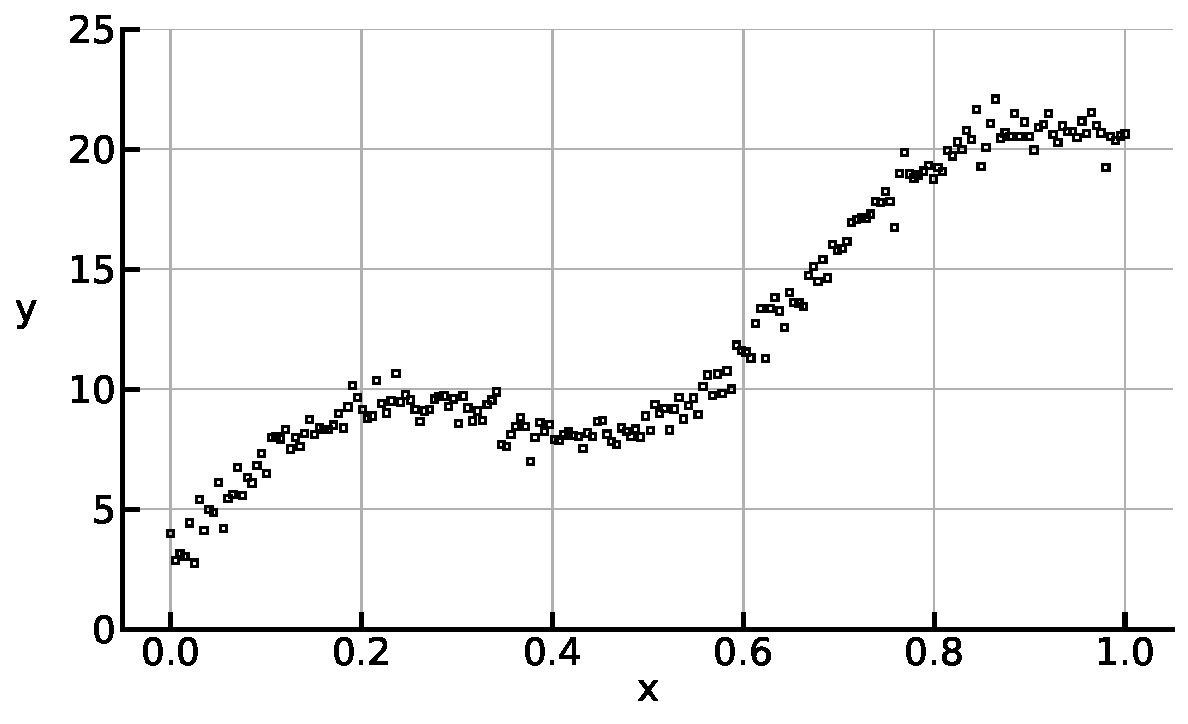
\includegraphics[width=\columnwidth]{thesisplots/test_func.pdf}
	\caption{Noisy samples determined from test function (\pref{fig:test_func})}
	\label{fig:test_func}
\end{figure}

%%%%%%%%%%%%%%%%%%%%%%%%%%%%%%%%%%%%%%%%%%%%%%%%%%%%%%%%%%%%%%%%%%%%%%%%%%%%%%%%%%%%%%%%%%%%%%%%%%%%%%%%%%%%%%%%%


\subsection{1d Function Estimation} \label{subsec:1d-function-estimation}

The goal is to model given data

\begin{align} \label{eq:data}
	\{\vec{x}, \vec{y}\} = \{x^{(i)}, y^{(i)}\}, \ i=1, 2, \dots, n 
\end{align}

using B-splines as basis functions. Theprefore, we want to estimate the unknown function $\vec{y} = f(\vec{x})$, which can be represented as a linear combination of $k$ B-spline basis functions $B_j^m$ of degree $m=3$, cf. (\pref{eq:bspline-bf-approach}), as

\begin{align} \label{eq:basis_function_approach}
	\vec{y} = \vec{X} \vec{\beta},
\end{align}

where $\vec{X} \in \mathbb{R}^{n\times k}$ is the B-spline basis matrix, cf. (\pref{eq:bspline-basis-matrix}), and $\vec{\beta} \in \mathbb{R}^k$ are the coefficients to be estimated. 

The least squares objective function to be minimized using the complete data is then given by

\begin{align} \label{eq:OF_1}
	Q_1(\vec{y}, \vec{\beta}) = \lVert \vec{y} - f(\vec{x}) \rVert^2 = \lVert \vec{y} - \vec{X}\vec{\beta} \rVert^2 
\end{align}	

The coefficients are determined ive function $Q_1$ given in (\pref{eq:OF_1}) with respect to $\vec{\beta}$, i.e.

\begin{align}\label{eq:optimization_problem_1}
	\hat{\vec{\beta}}_{LS} = \arg \min_{\vec{\beta}} Q_1(\vec{y}, \vec{\beta}).
\end{align}

Using the least squares algorithm LS, see Chapter \pref{subsubsec:Method-of-LS}, the minimization problem (\pref{eq:optimization_problem_1}) yields 

\begin{align} \label{eq:LS_coef}
	\hat{\vec{\beta}}_{LS}= (\transpose{\vec{X}} \vec{X})^{-1} \transpose{\vec{X}} \vec{y}.
\end{align} 


Figure \pref{fig:smooth_bf} shows a B-spline model using $k=10$ splines on an equidistant grid approximating the noisy data presented in Figure \pref{fig:test_func}, as well as the individual cubic ($m=3$) B-spline basis functions $B_i^3(\vec{x})$ multiplied with the corresponding, estimated coefficients $\hat{\vec{\beta}}_{LS, j} \ j=1, \dots, 10$.

\begin{figure}[H]
	\centering
	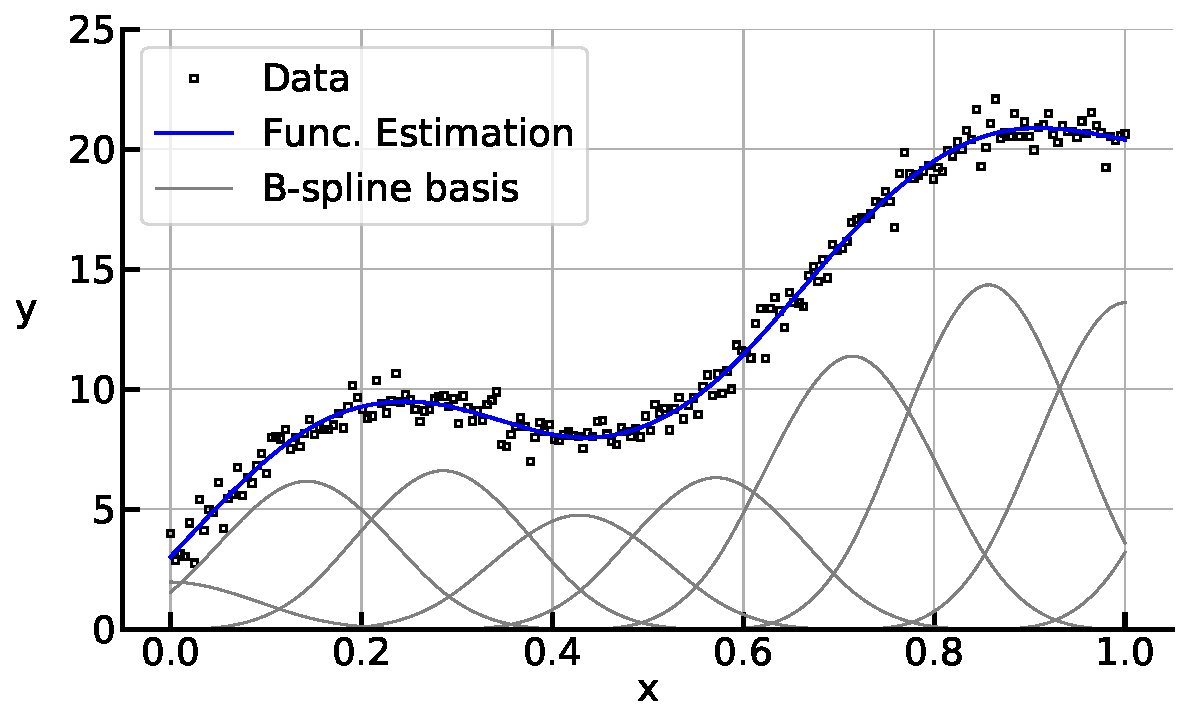
\includegraphics[width=\columnwidth]{thesisplots/smooth_bf.pdf}
	\caption{Approximation of the noisy data by B-splines without constraints}
	\label{fig:smooth_bf}
\end{figure}


Note, the number of splines $k$ has a strong influence on the amount of smoothing. A small number $k$ leads to a very smooth estimate, but a large data error. On the other hand, when the number of splines is relatively large, the data error is very small but the smoothness of the estimate is poor. This behavior is an example of the well-known bias-variance dilemma and depicted in Figure \pref{fig:smooth_bf_large}. \cite{sammut2011}
Here, two B-splines models with $k=10$ and $k=50$ are illustrated, which are applied to the noisy data shown in Figure \pref{fig:test_func}. To overcome this challenges, the B-splines will be extended by penalizing the second derivative of the estimation, see Chapter \pref{subsec:1D_smooth}. 

\begin{figure}[H]
	\centering
	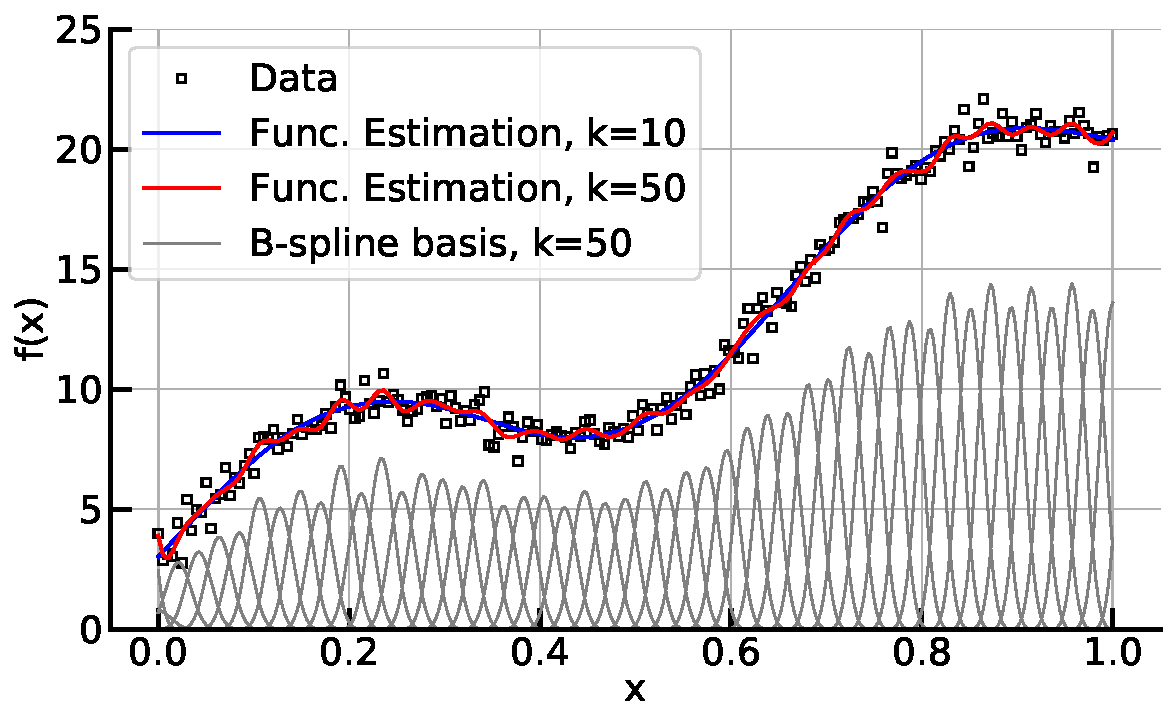
\includegraphics[width=\linewidth]{thesisplots/smooth_wiggly_bf.pdf}
	\caption{Approximation of the noisy data by 10 and 50 B-splines without constraints}
	\label{fig:smooth_bf_large}
\end{figure}


%%%%%%%%%%%%%%%%%%%%%%%%%%%%%%%%%%%%%%%%%%%%%%%%%%%%%%%%%%%%%%%%%%%%%%%%%%%%%%%%%%%%%%%%%%%%%%%%%%%%%%%%%%%%%%%%%
\subsection{1d Smooth Function Estimation} \label{subsec:1D_smooth}

The second derivative of the estimated function $f(x)$, i.e. $f''(x) = \sum_{j=1}^k B''_i(x) \beta_k$, has to be penalized to realize a smoother estimate when using  a high number of splines. Eilers and Marx have introduced the so-called P-splines. \cite{eilers1996flexible}, see Chapter \pref{subsec:p-splines}. Theprefore, the objective function in (\pref{eq:OF_1}) is extended by an additional term considering the smoothness, i.e.

\begin{align}\label{eq:OF_2}
	Q_2(\vec{y}, \vec{\beta}) = Q_1(\vec{y}, \vec{\beta}) + \lambda_s \mathcal{J}_s(\vec{\beta}; d) = \lVert \vec{y} - \vec{X} \vec{\beta} \rVert^2 + \lambda_s \transpose{\vec{\beta}} \transpose{\vec{D}}_d \vec{D}_d \vec{\beta}, 
\end{align}

with the smoothing parameter $\lambda_s$ and an appropriate mapping matrix $\vec{D}_d$ capturing the second derivative, which itself is a measure for function wiggliness. Here, an approximation of the second derivative can be performed by the squared finite difference of order $d$ of adjacent coefficients using the matrix form $\vec{D}_d$ of the difference operator of order $d$, see Chapter \pref{subsec:p-splines}. 

By minimizing the objective function (\pref{eq:OF_2}), i.e.

\begin{align}\label{eq:optimization_problem_2}
	\hat{\vec{\beta}}_{PLS} = \arg \min_{\vec{\beta}} Q_2(\vec{y}, \vec{\beta}),
\end{align}

using the penalized least squares algorithm PLS, the penalized least squares estimates are given by

\begin{align} \label{eq:PLS_coef}
	\hat{\vec{\beta}}_{PLS}= (\transpose{\vec{X}} \vec{X} + \lambda_s \transpose{\vec{D}}_d \vec{D}_d)^{-1} \transpose{\vec{X}} \vec{y}.
\end{align} 
%
In (\pref{eq:PLS_coef}), the smoothing parameter $\lambda_s$ plays a critical role and can be optimized using the information criteria specified in Chapter \pref{subsec:MAC}, e.g. AIC and BIC, or by using cross-validation techniques, see Chapter \pref{subsubsec:Cross-validation}. \cite{fahrmeir2007regression}

For small values $\lambda_s \rightarrow 0$, the penalized least squares estimate $\hat{\vec{\beta}}_{PLS}$ approaches the least squares estimate $\hat{\vec{\beta}}_{LS}$, cf. (\pref{eq:LS_coef}), while for large values $\lambda_s \gg 0$, the fitted function shows the behavior of a polynomial with $d-1$ degrees of freedom. For example, using $d=2$ and a large smoothing parameter $\lambda_s$ this configuration leads to a linear function, while using $d=1$ would lead to a constant function. \cite{fahrmeir2007regression}

Figure \pref{fig:psplines} shows the behavior of P-splines of degree $m=3$ using $k=50$ splines for several values of the smoothing parameter $\lambda_s = \{10^{-2}, 10^{2},10^{5},10^{6}\}$ and a smoothness penalty of order $d=2$.  As the value of $\lambda_s$ gets larger, the fitted curve becomes more smooth and thus the $2^{nd}$ derivative of the curve becomes smaller due to the penalty considered in the estimation, see (\pref{eq:PLS_coef}). For very large values of $\lambda_s$, the estimate approaches a straight line, see the yellow curve in Figure \pref{fig:psplines}.

\begin{figure}[H]
	\centering
	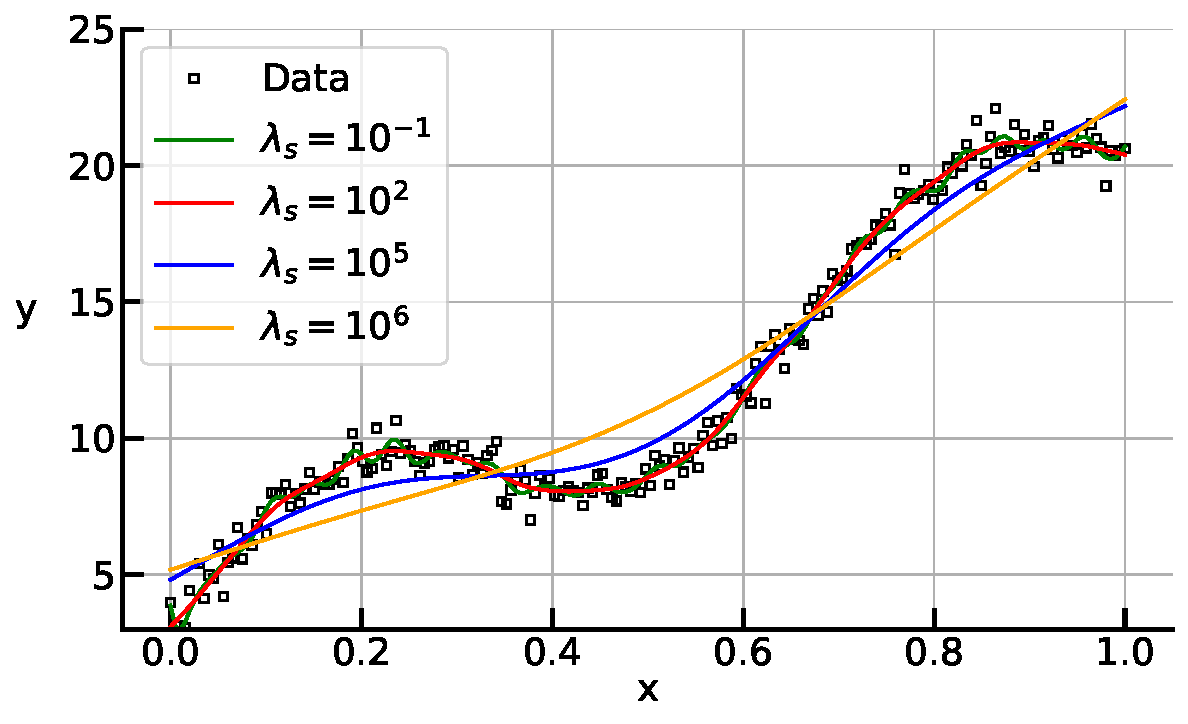
\includegraphics[width=\linewidth]{thesisplots/p_splines.pdf}
	\caption{Smooth function estimation for different smoothing parameters $\lambda_s$}
	\label{fig:psplines}
\end{figure}

%%%%%%%%%%%%%%%%%%%%%%%%%%%%%%%%%%%%%%%%%%%%%%%%%%%%%%%%%%%%%%%%%%%%%%%%%%%%%%%%%%%%%%%%%%%%%%%%%%%%%%%%%%%%%%%%%
\subsection{1d Constraint Function Estimation}
%%%%%%%%%%%%%%%%%%%%%%%%%%%%%%%%%%%%%%%%%%%%%%%%%%%%%%%%%%%%%%%%%%%%%%%%%%%%%%%%%%%%%%%%%%%%%%%%%%%%%%%%%%%%%%%%%
%%%%%%%%%%%%%%%%%%%%%%%%%%%%%%%%%%%%%%%%%%%%%%%%%%%%%%%%%%%%%%%%%%%%%%%%%%%%%%%%%%%%%%%%%%%%%%%%%%%%%%%%%%%%%%%%%	
\section{User-defined Constraints} \label{sec:user-defined-constraints}

As stated before, a priori domain knowledge given in Table \pref{tab:constraint_overview} can be introduced by the choice of the mapping matrix $\vec{D}_c$ and the weighting matrix $\vec{V}$, cf. (\pref{eq:mapping_matrix}) and (\pref{eq:PLS,c_coef}). Now a description of the different matrices, which are used to enforce the a priori known domain behavior, is presented. 

%%%%%%%%%%%%%%%%%%%%%%%%%%%%%%%%%%%%%%%%%%%%%%%%%%%%%%%%%%%%%%%%%%%%%%%%%%%%%%%%%%%%%%%%%%%%%%%%%%%%%%%%%%%%%%%%%
\subsection{Monotonicity Constraint}

The mapping matrix $\vec{D}_{monoton}$ enforcing monotonic behavior is given by the first order difference operator $\Delta^1$ for equidistant knot placement, cf. \pref{eq:d1-difference-matrix}. The corresponding matrix for $k$ splines is given as

\begin{align} \label{eq:D_c_monoton}
	\vec{D}_{monoton} = \begin{pmatrix}  -1 & 1  &  		& \\ 
		& -1 & 1 		& \\ 
		&    & \ddots  & \ddots  
	\end{pmatrix} \in \mathbb{R}^{k-1 \times k}.
\end{align}

The difference between monotonic increasing and decreasing behavior is controlled by the weighting matrix $\vec{V}$. For increasing behavior, the weighting matrix $\vec{V}$ is given by the weights $v_j$ according to

\begin{align} \label{eq:v_monoton_inc}
	v_j(\vec{\beta}) = \begin{cases}
			0, \quad \text{if} \ \Delta^1\beta_j \ge 0 \\ 
			1, \quad \text{if} \ \Delta^1\beta_j < 0
	\end{cases}	\ \text{for} \ j=2, \dots, k-1.
\end{align}

For decreasing behavior, the weighting matrix $\vec{V}$ is given by the weights $v_j$ according to
\begin{align} \label{eq:v_monoton_dec}
	v_j(\vec{\beta}) = \begin{cases} 0, \quad \text{if} \ \Delta^1\beta_j \le 0 \\ 
		1, \quad \text{if} \ \Delta^1\beta_j > 0
	\end{cases} \ \text{for} \ j=2, \dots, k-1.
\end{align}

This states, that the penalty term $\mathcal{J}_c(\vec{\beta}; c)$ only contributes if adjacent coefficients $\beta_{j-1}$ and $\beta_j$ are increasing or decreasing, respectively. \cite{hofner2011monotonicity} \cite{eilers2005unimodal}

%%%%%%%%%%%%%%%%%%%%%%%%%%%%%%%%%%%%%%%%%%%%%%%%%%%%%%%%%%%%%%%%%%%%%%%%%%%%%%%%%%%%%%%%%%%%%%%%%%%%%%%%%%%%%%%%%	
\subsection{Curvature Constraint}

In the simplest case, the curvature of the function $f(x)$ can either be convex, i.e. $f''(x) \ge 0$, or concave, i.e. $f''(x) \le 0$. The mapping matrix $\vec{D}_{curvature}$ enforcing this behavior can be approximated by the second order difference operator $\Delta^2$ for equidistant knot placement, cf. (\pref{eq:d2-difference-matrix}). The corresponding matrix for $k$ splines is given as

\begin{align} \label{eq:D_c_curvature}
	\vec{D}_{curvature} = \begin{pmatrix} 1 & -2 & 1 		&  		 & \\ 
		& 1  &-2 	    &1 		 & \\
		& 	  & \ddots  & \ddots & \ddots  
	\end{pmatrix} \in \mathbb{R}^{k-2 \times k}.
\end{align}	

The difference between concave and convex curvature is controlled by the weighting matrix $\vec{V}$. For concave curvature, the weighting matrix $\vec{V}$ is given by the weights $v_j$ according to

\begin{align}\label{eq:v_curvature_concave}
	v_j(\vec{\beta}) = \begin{cases} 
		0, \quad \text{if} \ \Delta^2\beta_j \le 0 \\ 
		1, \quad \text{if} \ \Delta^2\beta_j > 0
	\end{cases} \ \text{for} \ j=1, \dots, k-2.
\end{align}

For convex curvature, the weighting matrix $\vec{V}$ is given by the weights $v_j$ according to

\begin{align}\label{eq:v_curvature_convex}
	v_j(\vec{\beta}) = \begin{cases} 
		0, \quad \text{if} \ \Delta^2\beta_j \ge 0 \\ 
		1, \quad \text{if} \ \Delta^2\beta_j < 0
	\end{cases}\ \text{for} \ j=1, \dots, k-2.
\end{align}	

Theprefore, the penalty term $\mathcal{J}_c(\vec{\beta}; c)$ in (\pref{eq:OF_3}) or (\pref{eq:PLS,c_coef}) only contributes if the second order difference of adjacent coefficients $\vec{\beta}$ is either positive or negative, respectively. \cite{eilers2005unimodal}

%%%%%%%%%%%%%%%%%%%%%%%%%%%%%%%%%%%%%%%%%%%%%%%%%%%%%%%%%%%%%%%%%%%%%%%%%%%%%%%%%%%%%%%%%%%%%%%%%%%%%%%%%%%%%%%%%	
\subsection{Unimodality Constraint}

We assume that there is a peak in the data $\{x^{(i)}, y^{(i)}\}$ and theprefore want to constrain the fit to include a peak. The peak constraint is given by the unimodal mapping matrix $D_{unimodal}$ and the peak weighting matrix $V$. A function $f(x)$ is said to be unimodal if for some value $m$, it is monotonically increasing for $x \le m$ and monotonically decreasing for $x \ge m$. 

The mapping matrix $\vec{D}_{unimodal}$ enforcing unimodal behavior can be constructed using the first order difference operator $\Delta^1$ for equidistant knot placement, cf. (\pref{eq:d1-difference-matrix}), and is given for $k$ splines as 

\begin{align}\label{eq:D_c_unimodal}
	\vec{D}_{unimodal} = \begin{pmatrix} -1 & 1 \\ 
		& \ddots & \ddots  \\
		& & -1 & 1
	\end{pmatrix} \in \mathbb{R}^{k-1 \times k}
\end{align}

The weighting matrix $\vec{V}$ now has a special structure. First, we construct the B-spline basis using the given data as in Chapter \pref{subsec:b-splines}. We then need to find the index $j_{peak}$ of the \emph{peak spline}, which has the maximal value at the peak data point $\max \{f(x^{(i)}) \ \forall \ i \}$, see Figure \pref{fig:peak_spline}. The index $j_{peak}$ is now used as splitting point for the weighting matrix $\vec{V}$. All coefficients $\beta_j$ for $j < j_{peak}$ are constrained to be monotonic increasing, i.e. $\Delta^1 \beta_j \ge 0$ for $j = 1, \dots, j_{peak}-1$, while all coefficients $\beta_j$ for $j > j_{peak}$ are constrained to be monotonic decreasing, i.e. $\Delta^1 \beta_j \le 0$ for $j = j_{peak}+1, \dots, k$. The coefficient $\beta_{j_{peak}}$ stays unconstrained. \cite{eilers2005unimodal} 

\begin{figure}[H]
	\centering
	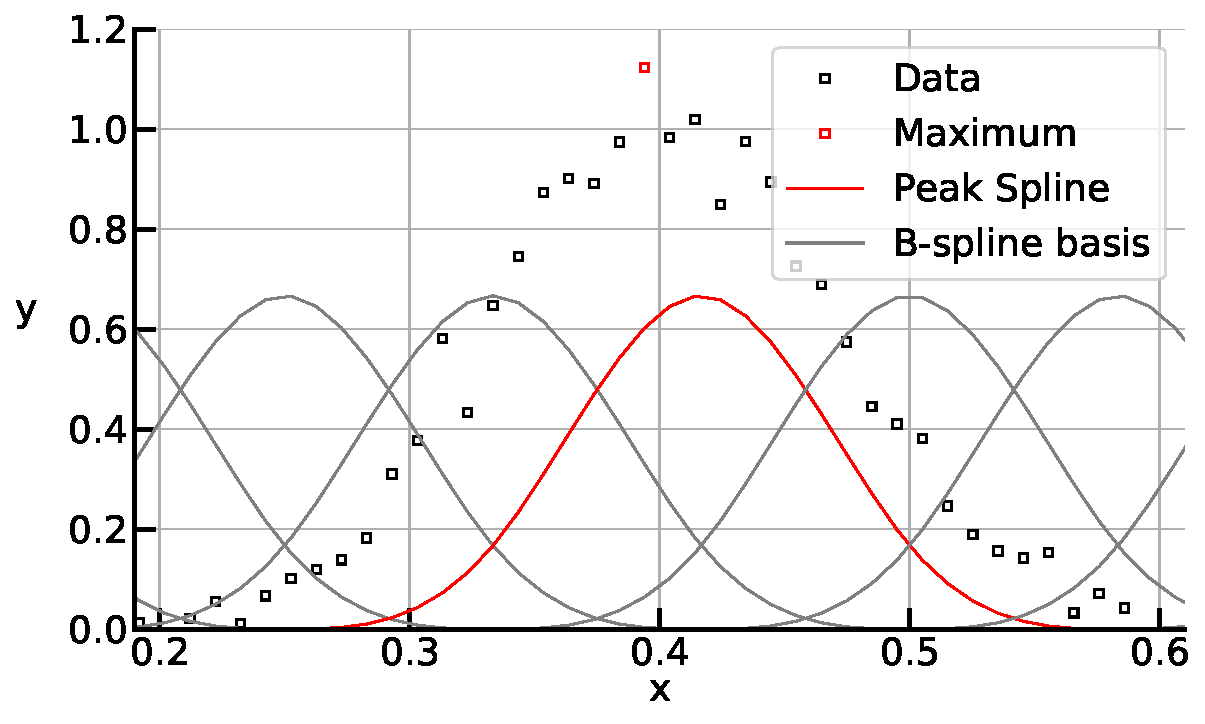
\includegraphics[width=\linewidth]{thesisplots/peak_spline.pdf}
	\caption{Identification of the peak spline based on data}
	\label{fig:peak_spline}
\end{figure}


The weights $v_j$ to incorporate the peak constraint have the following structure, i.e.

\begin{align}\label{eq:v_peak_1}
	v_j(\vec{\beta}) &= \begin{cases} 
		0, \quad \text{if} \ \Delta^1\beta_j \ge 0 \\ 
		1, \quad \text{if} \ \Delta^1\beta_j  < 0
	\end{cases}, \quad \text{for} \ j=2, \dots, j_{peak}-1
\end{align}

and 

\begin{align}\label{eq:v_peak_2}
	v_j(\vec{\beta}) &= \begin{cases} 
		0, \quad \text{if} \ \Delta^1\beta_j \le 0 \\ 
		1, \quad \text{if} \ \Delta^1\beta_j > 0
	\end{cases}, \quad \text{for} \ j=j_{peak}+1, \dots, k.
\end{align}

The weight $v_{j_{peak}}$ for the \emph{peak spline} is given by $v_{j_{peak}}(\vec{\beta}) = 0$. 

When assuming a valley in the data, the same approach as above can easily be used by multiplying the data with $-1$ or by always doing the inverse operation, i.e. finding the index $j_{valley}$ of the \emph{valley spline}, then constraining all splines for $j < j_{valley}$ to be monotonic decreasing, i.e. $\Delta^1 \beta_j \le 0$ for $j = 1, \dots, j_{valley}-1$, and all splines for $j > j_{valley}$ to be monotonic increasing, i.e. $\Delta^1 \beta_j \ge 0$ for $j = j_{valley}+1, \dots, k$. The coefficient $\beta_{j_{valley}}$ stays unconstrained. 

The weights $v_j$ to consider a valley constraint are given by

\begin{align}\label{eq:v_valley_1}
	v_j(\vec{\beta}) &= \begin{cases} 
		0, \quad \text{if} \ \Delta^1\beta_j \le 0 \\ 
		1, \quad \text{if} \ \Delta^1\beta_j > 0
	\end{cases}, \quad \text{for} \ j=2, \dots, j_{valley}-1
\end{align}

and 

\begin{align}\label{eq:v_valley_2}
	v_j(\vec{\beta}) &= \begin{cases} 
		0, \quad \text{if} \ \Delta^1\beta_j \ge 0 \\ 
		1, \quad \text{if} \ \Delta^1\beta_j < 0.
	\end{cases}, \quad \text{for} \  j=j_{valley}+1, \dots, k.
\end{align}

The weight $v_{j_{valley}}$ for the \emph{valley spline} is given by $v_{j_{valley}}(\vec{\beta}) = 0$.

%%%%%%%%%%%%%%%%%%%%%%%%%%%%%%%%%%%%%%%%%%%%%%%%%%%%%%%%%%%%%%%%%%%%%%%%%%%%%%%%%%%%%%%%%%%%%%%%%%%%%%%%%%%%%%%%
\subsection{Boundedness Constraint}

For certain physical systems, it is known a priori that the measured quantity cannot be smaller than zero, i.e. $f(x) \ge 0$. Using data-driven modeling on noisy data can lead to predictions in the interpolation and extrapolation regime, which may not hold this constraint due to uncertainties captured by the data. It is theprefore appropriate to apply the user-defined constraint of boundedness from below.

The user-defined constraint for boundedness from below by $M=0$ uses as mapping matrix $\vec{D}_c$ the B-spline basis matrix $\vec{X} \in \mathbb{R}^{n \times k}$. The weighting matrix $\vec{V} \in \mathbb{R}^{n\times n}$, with individual weights $v_j$, is specified as follows:

\begin{align} \label{eq:v_boundedness}
	v_j(\vec{\beta}) = \begin{cases} 
		0, \quad \text{if} \ f(x^{(j)}) \ge M\\ 
		1, \quad \text{if} \ f(x^{(j)})  < M 		
	\end{cases} \text{for} \ j=1, \dots, n.
\end{align}

Using different values of $M$ allows us to bound from below from any number $M$. Switching the comparison operators in (\pref{eq:v_boundedness}) enables us to bound functions from above. 

%%%%%%%%%%%%%%%%%%%%%%%%%%%%%%%%%%%%%%%%%%%%%%%%%%%%%%%%%%%%%%%%%%%%%%%%%%%%%%%%%%%%%%%%%%%%%%%%%%%%%%%%%%%%%%%%
\subsection{Jamming Constraint}

Jamming the function $f(x)$ by some point $p = \{x^{(jamm)}, y^{(jamm)}\}$ means that the estimated function $f(x^{(jamm)}) \approx y^{(jamm)}$. This can be incorporated using the B-spline basis matrix $\vec{X} \in \mathbb{R}^{n \times k}$ as mapping matrix $\vec{D}_c$ and a weighting matrix $\vec{V} \in \mathbb{R}^{n \times n}$ given by

\begin{align} \label{eq:v_jamming}
	v_j(\vec{\beta}) = 
		\begin{cases}
			0, \quad \text{if} \ x^{(j)} \ne x^{(jamm)} \\
			1, \quad \text{if} \ x^{(j)} = x^{(jamm)} 
	\end{cases} \text{for} \ j = 1, \dots, n.
\end{align} 

%%%%%%%%%%%%%%%%%%%%%%%%%%%%%%%%%%%%%%%%%%%%%%%%%%%%%%%%%%%%%%%%%%%%%%%%%%%%%%%%%%%%%%%%%%%%%%%%%%%%%%%%%%%%%%%%
\subsection{Penalty Term for Tensor-Product Splines}

To extend the framework of mapping matrices to two dimensions and tensor-product splines, we again use the concept of Kronecker products given in Chapter \pref{subsubsec:tp-splines}. In principle, every possible pair of one dimensional user-defined constraints can be constructed using the approach in Chapter \pref{subsubsec:tp-splines}, e.g. unimodality in two dimensions would be obtained using the unimodal mapping matrix depicted above for each dimension. We then also need to include the constraint specific weight matrices $\vec{V}$.

The penalty term for the constraint given by $c_1$ for dimension $1$ and $c_2$ for dimension $2$ then has the form

\begin{align} \label{eq:J-c-tps}
	\mathcal{J}_c(\vec{\beta}; c) = \transpose{\vec{\beta}} \Big[ \vec{I}^2 \otimes \vec{K}_{c_1} + \vec{K}_{c_2} \otimes \vec{I}^1\Big] \vec{\beta}
\end{align}

with the respective penalty matrices $\vec{K}_{c_1} = \vec{D}_{c_1}^{\text{T}} \vec{V}_1 \vec{D}_{c_1}$ for dimension $x_1$ and $\vec{K}_{c_2} = \vec{D}_{c_2}^{\text{T}} \vec{V}_2 \vec{D}_{c_2}$ for dimension $x_2$ using the weighting matrices $\vec{V}_1$ and $\vec{V}_2$, the mapping matrices $\vec{D}_{c_1}$ and $\vec{D}_{c_2}$ and the identity matrices $\vec{I}^1$ and $\vec{I}^2$ for the respective dimension.

%%%%%%%%%%%%%%%%%%%%%%%%%%%%%%%%%%%%%%%%%%%%%%%%%%%%%%%%%%%%%%%%%%%%%%%%%%%%%%%%%%%%%%%%%%%%%%%%%%%%%%%%%%%%%%%%%
%%%%%%%%%%%%%%%%%%%%%%%%%%%%%%%%%%%%%%%%%%%%%%%%%%%%%%%%%%%%%%%%%%%%%%%%%%%%%%%%%%%%%%%%%%%%%%%%%%%%%%%%%%%%%%%%%
\section{n-d Constraint Function Estimation}

The extension from one input to multiple input dimensions uses the concept of additive models given in Chapter \pref{subsubsec:STAR}. Given input data $\{ x_1^{(i)}, \dots, x_q^{(i)}, y^{(i)}\}, \ i=1, 2, \dots, n$ and $q$ as the number of inputs, the combined model using all available B-splines and tensor-product splines is given, cf. (\pref{eq:STAR}), as

\begin{align} \label{eq:tps_all}
	y = f(x_1,..., x_q) = \sum_{j=1}^q s_j(x_j) + \sum_{j=1}^{q-1} \sum_{r>j}^q t_{j, r}(x_j, x_r)
\end{align}

where $s_j(x_j)$ is the B-spline estimate given by $s_j(x_j) = \vec{X}_{s_j} \vec{\beta}_{s_j}$ and $t_{j, r}(x_j,x_r)$ is the tensor-product estimate is given by $t_{j, r}(x_j,x_r) = \vec{X}_{t_{j,r}} \vec{\beta}_{t_{j, r}}$. The number of individual estimates is given by 

\begin{align}
	n_{total} = q + \frac{q(q-1)}{2}.  
\end{align}

The constrained penalized least squares objective function for additive models can now be written similar to (\pref{eq:OF_3}) as

\begin{align}\label{eq:OF_6}
	Q_6(\vec{y}, \vec{\beta}) = Q_1(\vec{y}, \vec{\beta}) + \transpose{\vec{\lambda}}_s	\vec{\mathcal{J}}_s(\vec{\beta}; \vec{d}) + \transpose{\vec{\lambda}}_c \vec{\mathcal{J}}_c(\vec{\beta}; \vec{c}).
\end{align}

with $\vec{\lambda}_s \in \mathbb{R}^{n_{total}}$ and  $\vec{\lambda}_c \in \mathbb{R}^{n_{total}}$  defined as vectors with one value of smoothness and constraint parameter for each individual estimate, respectively. 

We now need to specify the three parts of the objective function in (\pref{eq:OF_6}). 

%%%%%%%%%%%%%%%%%%%%%%%%%%%%%%%%%%%%%%%%%%%%%%%%%%%%%%%%%%%%%%%%%%%%%%%%%%%%%%%%%%%%%%%%%%%%%%%%%%%%%%%%%%%%%%%%%
\subsection{Data Term}

Assuming the use of $k$ splines for the B-spline estimates and $k^2$ splines for the tensor-product estimates, the total number of coefficients to be determined is given by 

\begin{align}\label{eq:tps_total_number_of_coef}
	k_{total} = qk + \frac{q(q-1)}{2}k^2. 
\end{align}

Since all B-spline and tensor-product spline models follow a linear model structure, see Chapter \pref{subsec:b-splines} and \pref{subsubsec:tp-splines}, we can combine them into one large model, cf. (\pref{eq:STAR-block-diag}), given by

\begin{align}\label{eq:tps_lin_mod}
	\vec{y} = \vec{X} \vec{\beta}
\end{align}

where the matrix $\vec{X} \in \mathbb{R}^{n \times k_{total}}$ is given in (\pref{eq:STAR-block-diag}) as horizontal concatenation of the individual bases and the combined coefficient vector $\vec{\beta} \in \mathbb{R}^{k_{total}}$ is given in (\pref{eq:STAR-block-diag}) by a vertical concatenation of the individual coefficient vectors. 

The data term $Q_1(\vec{y}, \vec{\beta})$ in the constrained penalized least squares objective function given in (\pref{eq:OF_6}) can now be evaluated using arbitrary input dimensions. 

%%%%%%%%%%%%%%%%%%%%%%%%%%%%%%%%%%%%%%%%%%%%%%%%%%%%%%%%%%%%%%%%%%%%%%%%%%%%%%%%%%%%%%%%%%%%%%%%%%%%%%%%%%%%%%%%%
\subsection{Smoothness Term}

The combined smoothness penalty term $\vec{\mathcal{J}}_s(\vec{\beta}; \vec{d}) \in \mathbb{R}^{n_{total}}$ is then given as

\begin{align}\label{eq:J_s_ndim}
	\vec{\mathcal{J}}_s(\vec{\beta}; \vec{d}) &= 
	\begin{pmatrix}
		\mathcal J_{s_1}(\vec{\beta}_{s_1}; d_{s_1}) \\ 
		\vdots \\ 
		\mathcal J_{s_q}(\vec{\beta}_{s_q}; d_{s_q}) \\
		\mathcal J_{t_{1,2}}(\vec{\beta}_{t_{1,2}}; d_{t_{1,2}}) \\
		\vdots \\
		\mathcal J_{t_{q-1,q}}(\vec{\beta}_{t_{q-1,q}}; d_{t_{q-1,q}}) \\
	\end{pmatrix}
\end{align}

with $\mathcal J_e(\vec{\beta}_e; d_e) = \transpose{\vec{\beta}}_e \transpose{\vec{D}}_{d_e} \vec{D}_{d_e} \vec{\beta}_e$ determining the smoothness penalty term using the coefficients $\vec{\beta}_e$ and mapping matrix $\vec{D}_{d_e}$, see Chapter \pref{subsec:p-splines} and Chapter \pref{subsubsec:tp-splines}, for each estimate $e \in \{s_1, \dots, s_q, t_{1,2}, \dots, t_{q-1,q}\}$. The vector $\vec{d} \in \mathbb{R}^{n_{total}}$ consists of the orders $d_e$ determining the mapping matrix $\vec{D}_{d_e}$ of the smoothness constraint for each individual estimate $e$. 

%%%%%%%%%%%%%%%%%%%%%%%%%%%%%%%%%%%%%%%%%%%%%%%%%%%%%%%%%%%%%%%%%%%%%%%%%%%%%%%%%%%%%%%%%%%%%%%%%%%%%%%%%%%%%%%%%
\subsection{Constraint Term}
The combined constraint penalty term $\vec{\mathcal{J}}_c(\vec{\beta}; \vec{c}) \in \mathbb{R}^{n_{total}}$ is then given as

\begin{align}\label{eq:J_c_ndim}
	\vec{\mathcal{J}}_c(\vec{\beta}; \vec{c}) &= 
	\begin{pmatrix}
		\mathcal J_{s_1}(\vec{\beta}_{s_1}; c_{s_1}) \\ 
		\vdots \\ 
		\mathcal J_{s_q}(\vec{\beta}_{s_q}; c_{s_q}) \\
		\mathcal J_{t_{1,2}}(\vec{\beta}_{t_{1,2}}; c_{t_{1,2}}) \\
		\vdots \\
		\mathcal J_{t_{q-1,q}}(\vec{\beta}_{t_{q-1,q}}; c_{t_{q-1,q}}) \\
	\end{pmatrix}
\end{align}

with $\mathcal J_e(\vec{\beta}_e; c_e) = \transpose{\vec{\beta}}_e \transpose{\vec{D}}_{c_e} \vec{V}_{c_e} \vec{D}_{c_e} \vec{\beta}_e$ determining the constraint penalty term using the coefficients $\vec{\beta}_e$, the mapping matrix $\vec{D}_{c_e}$ and the weighting matrix $\vec{V}_e$ for each estimate $e \in \{s_1, \dots, s_q, t_{1,2}, \dots, t_{q-1,q}\}$, see Chapter (\pref{sec:user-defined-constraints}). The vector $\vec{c} \in \mathbb{R}^{n_{total}}$ consists of the constraint type $c_e$, e.g. monoton increasing, determining the mapping matrix $\vec{D}_{c_e}$ for each individual estimate $e$. 

%%%%%%%%%%%%%%%%%%%%%%%%%%%%%%%%%%%%%%%%%%%%%%%%%%%%%%%%%%%%%%%%%%%%%%%%%%%%%%%%%%%%%%%%%%%%%%%%%%%%%%%%%%%%%%%%%

The objective function (\pref{eq:OF_6}) is then optimized, i.e.

\begin{align}\label{eq:optimization_problem_6}
	\hat{\vec{\beta}}_{PLS,c,nd} = \arg \min_{\vec{\beta}} Q_6(\vec{y}, \vec{\beta}),
\end{align}

using the penalized iteratively reweighted least squares algorithm, cf. (\pref{eq:PLS,c_coef}), to obtain the coefficients $\hat{\vec{\beta}}_{PLS,c,nd}$ as

\begin{align} \label{eq:beta-pls-c-nd-formula}
	\hat{\vec{\beta}}_{PLS,c,nd} = (\transpose{\vec{X}} \vec{X} +\vec{K}_s + \vec{K}_c)^{-1} \transpose{\vec{X}} \vec{y}. 
\end{align}

In (\pref{eq:beta-pls-c-nd-formula}), $\vec{X} \in \mathbb{R}^{n \times k_{total}}$ is the combined basis matrix, cf. (\pref{eq:STAR-block-diag}), $\vec{K}_s \in \mathbb{R}^{k_{total} \times k_{total}}$ is the combined smoothness matrix given as

\begin{align} \label{eq:combined-smoothness-matrix}
	\vec{K}_s = \rotatebox{-90}{$\begin{pmatrix} 
					\lambda_{s_1} \transpose{\vec{D}_{d_{s_1}}} \vec{D}_{d_{s_1}} & 0 \\
					 							0 						  &	\ddots & 0 \\
					 													  &  0 	   & \lambda_{s_q} \transpose{\vec{D}_{d_{s_q}}} \vec{D}_{d_{s_q}} & 0 \\
					 													  &        &           0										   & \lambda_{s_{1,2}} \transpose{\vec{D}_{d_{t_{1,2}}}} \vec{D}_{d_{t_{1,2}}} & 0 \\
					 													  &  & &    0 & \ddots & 0 \\
					 													  &  & &      &   0    & \lambda_{s_{q-1,q}} \transpose{\vec{D}_{d_{t_{q-1,q}}}} \vec{D}_{d_{t_{q-1,q}}}
			\end{pmatrix}$} 
\end{align}

and $\vec{K}_c \in \mathbb{R}^{k_{total} \times k_{total}}$ is the combined constraint matrix as 

\begin{align} \label{eq:combined-constraint-matrix}
	\vec{K}_c = \rotatebox{-90}{$\begin{pmatrix} 
					\lambda_{c_1} \transpose{\vec{D}_{c_{s_1}}} \vec{V}_{c_{s_1}} \vec{D}_{c_{s_1}} & 0 \\
													 			0 						& \ddots & 0 \\
													 			                 		&  0 	 & \lambda_{c_q} \transpose{\vec{D}_{c_{s_q}}} \vec{V}_{c_{s_q}} \vec{D}_{c_{s_q}} & 0 \\
													 			                 		&        &           0										    & \lambda_{c_{1,2}} \transpose{\vec{D}_{c_{t_{1,2}}}} \vec{V}_{c_{t_{1,2}}} \vec{D}_{c_{t_{1,2}}} & 0 \\
													 			                 		& &  &   0 & \ddots & 0 \\
																			         	& &  & 	   &	0   & \lambda_{c_{q-1,q}} \transpose{\vec{D}_{c_{t_{q-1,q}}}} \vec{V}_{c_{t_{q-1,q}}} \vec{D}_{c_{t_{q-1,q}}}
	\end{pmatrix}$}. 
\end{align}




%%%%%%%%%%%%%%%%%%%%%%%%%%%%%%%%%%%%%%%%%%%%%%%%%%%%%%%%%%%%%%%%%%%%%%%%%%%%%%%%%%%%%%%%%%%%%%%%%%%%%%%%%%%%%%%%%%%
\subsection{2-d Example} \label{subsec:2d-example}

As example for the n-d constraint function estimation, we take a look at the function 

\begin{align} \label{eq:2d_test_func}
	f(x_1, x_2) = 2\exp{\Big(-\frac{(x_1 - 0.25)^2}{0.08}\Big)} + x_2^2 + \eta
\end{align}

for $x_1 \in [0,1]$ and $x_2 \in [0,1]$ and random Gaussian noise $\eta$ with $\sigma_{noise} = 0.1$. Theprefore we expect a peak in dimension $x_1$ as well as increasing behavior for dimension $x_2$, see Figure \pref{fig:2d_example}. The user-defined constraints are theprefore $c_1 = \text{unimodal}$ and $c_2 = \text{monotonic increasing}$ Using this knowledge, we create a model with the following characteristics:

\begin{itemize}
	\item B-spline smooth $s_1(x_1)$: $k_{x_1} = 50$, $c = c_1$, $\lambda_s = 1$ and $\lambda_c = 6000$
	\item B-spline smooth $s_2(x_2)$: $k_{x_2} = 50$, $c = c_2$, $\lambda_s = 1$ and $\lambda_c = 6000$
\end{itemize}

The fit for this model as well as the individual estimates $s_1(x_1)$ and $s_2(x_2)$ are shown in Figure \pref{fig:2d_example}. The model fits the data quite well and holds the specified constraints for the individual dimensions.

\begin{figure}[H]
	\centering
	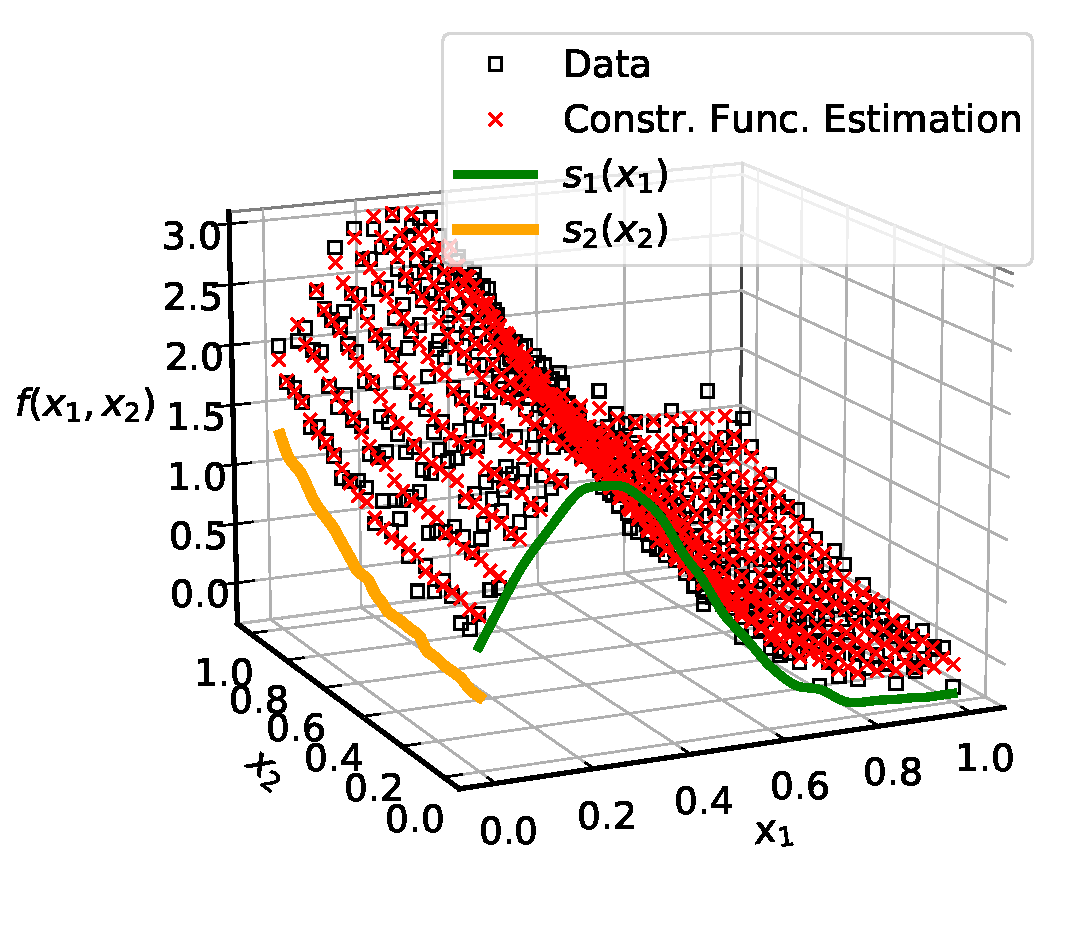
\includegraphics[width=\linewidth]{thesisplots/2d_example.pdf}
	\caption{2-d test function for n-d constrained function estimation}
	\label{fig:2d_example}
\end{figure}

\end{comment}

